\input{header_xe.tex}
\def \labnum {3}
\def \labsubj {Теория автоматов}
\def \labauthor {Чебыкин И. Б.}
\def \labgroup {P3301}
\def \labinsp {Ожиганов А. А.}
\def \labname {Канонический метод структурного синтеза \\ Вариант: 1}
\isnametrue

\usepackage{listings,longtable,amsmath,amsfonts,graphicx,tikz,tabularx,pgf,multirow}
\usepackage{caption}
\usepackage{float}
\usetikzlibrary{arrows,automata}

\captionsetup{labelsep=period}
\pagestyle{fancy}
\begin{document}
\input{title.tex}

\section{Описание работы}
Цель -- практическое освоение метода перехода от абстрактного
автомата к структурному автомату

Абстрактный автомат задан табличным способом. Причем
абстрактный автомат Мили представлен таблицами переходов и
выходов, а абстрактный автомат Мура - одной отмеченной таблицей
переходов. Для синтеза структурного автомата использовать
функционально полную систему логических элементов И, ИЛИ, НЕ и
автомат Мура, обладающий полнотой переходов и полнотой выходов.
Синтезированный структурный автомат представить в виде ПАМЯТИ и
КОМБИНАЦИОННОЙ СХЕМЫ.

\section{Выполнение}
\subsection{Исходный автомат}

\begin{table}[!h]
\begin{tabular}{|c|c|c|c|c|c|c|c|}
\hline
$\delta$  & $a_1$ & $a_2$ & $a_3$ & $\lambda$ & $a_1$ & $a_2$ & $a_3$ \\ \hline
$z_1$     & $a_2$ & $a_3$ & $a_1$ & $z_1$     & $w_2$ & $w_2$ & $w_1$ \\ \hline
$z_2$     & $a_1$ &       & $a_2$ & $z_2$     & $w_1$ &       & $w_2$ \\ \hline
\end{tabular}
\end{table}
\subsection{Переход к структурному автомату}

\paragraph{Кодирование входных и выходных сигналов}\mbox{}\\

Закодируем входные сигналы:

\begin{table}[!h]
\begin{tabular}{|c|c|}
\hline
$T_1$ & $X_1$ \\ \hline
$Z_1$ & $0$ \\ \hline
$Z_2$ & $1$ \\ \hline
\end{tabular}
\end{table}

Для минимизации произведем следующие вычисления:

$W_1 = 2$

$W_2 = 3$

Закодируем выходной сигнал с наибольшим числом повторений как 0 и другой как 1:

\begin{table}[!h]
\begin{tabular}{|c|c|}
\hline
$T_2$ & $Y_1$ \\ \hline
$W_2$ & $0$ \\ \hline
$W_1$ & $1$ \\ \hline
\end{tabular}
\end{table}

\paragraph{Кодирование состояний автомата и получение таблицы переходов}\mbox{}\\

Посчитаем количество переходов в состояние автомата и согласно
упорядоченному по убыванию списку закодируем состояния автомата:
\begin{table}[H]
\begin{tabular}{|c|c|c|}
\hline
$T_3$ & $Q_1$ & $Q_2$  \\ \hline
$a_1$ & $0$ & $0$  \\ \hline
$a_2$ & $0$ & $1$  \\ \hline
$a_3$ & $1$ & $0$  \\ \hline
\end{tabular}
\end{table}

По таблицам с исходными данными и таблицам 1 – 3 строим таблицу
переходов и таблицу выходов структурного автомата.

$P_1P_2 = \delta(Q_1Q_2x_1)$

\begin{table}[H]
\begin{tabular}{|c|c|c|c|}
\hline
$T_4\quad x_1 \backslash Q_1Q_2$ & $00$ & $01$ & $10$ \\ \hline
$0$          & $01$ & $10$ & $00$ \\ \hline
$1$          & $00$ & $- $ & $01$  \\ \hline
\end{tabular}
\end{table}


$y_1 = \lambda(Q_1Q_2x_1)$


\begin{table}[H]
\begin{tabular}{|c|c|c|c|}
\hline
$T_5\quad x_1 \backslash Q_1Q_2$ & $00$ & $01$ & $10$ \\ \hline
$0$          & $0$ & $0$ & $1$ \\ \hline
$1$          & $1$ & $- $ & $0$  \\ \hline
\end{tabular}
\end{table}

$y_1 = 1 \vee 4$

\paragraph{RS-триггер}\mbox{}\\

По таблице 4, согласно таблицам 1-3 строим таблицу функции
переключения RS-триггера:

$R_1S_1R_2S_2 = \mu(Q_1Q_2x_1)$

\begin{table}[!h]
\begin{tabular}{|c|c|c|c|c|c|c|}
\hline
$x_1 \backslash Q_1Q_2$ & $0$ & $0$ & $0$ & $1$ & $1$ & $0$ \\ \hline
$0$          & $-0$ & $01$ & $01$ & $10$ & $10$ & $-0$ \\ \hline
$1$          & $-0$ & $-0$ & $- $ & $- $ & $10$ & $01$  \\ \hline
\end{tabular}
\end{table}

ДНФ:

$R1 = 4 \vee 5$

$S1 = 2$

$R2 = 2$

$S2 = 0 \vee 5$

В итоге для RS-триггера получаем:

$y1 = 1 \vee 4$

$R1 = 4 \vee 5$

$S1 = 2$

$R2 = 2$

$S2 = 0 \vee 5$

Синтезированный структурный автомат в виде комбинационной схемы и памяти:

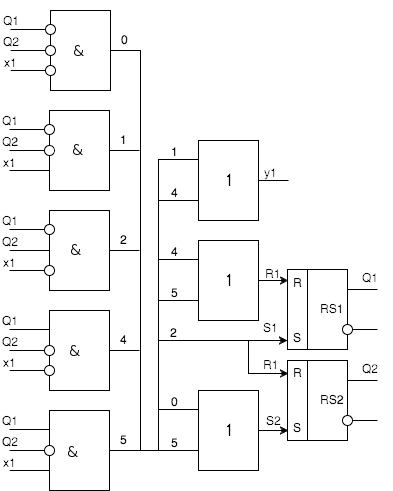
\includegraphics{img/rs.png}

Проверка:
\begin{table}[!h]
\tiny
\resizebox{\textwidth}{!}{\begin{tabular}{|c|c|c|c|c|c|c|c|c|}
\hline
\multicolumn{2}{|c|}{Входящий сигнал}        &         & z2 (1)  & z1 (0)  & z1 (0)  & z2 (1)  & z1 (0)  & z1 (0) \\ \hline
\multirow{2}{*}{Состояние}            & Исх. & a1 (00) & a1 (00) & a2 (01) & a3 (10) & a2 (01) & a3 (10) & a1 (00) \\ \cline{2-9}
                                      & Тр.  &         & 00      & 01      & 10      & 01      & 10      & 00 \\ \hline

\multirow{2}{*}{Выходящий сигнал}     & Исх. &         & w1 (1)  & w2 (0)  & w2 (0)  & w2 (0)  & w2 (0)  & w1 (1) \\ \cline{2-9}
                                      & Тр.  &         & 1       & 0       & 0       & 0       & 0       & 0 \\ \hline
\end{tabular}}
\end{table}

\paragraph{JK-триггер}\mbox{}\\

По таблице 4, согласно таблицам 1-3 строим таблицу функции
переключения JK-триггера:

$J_1K_1J_2K_2 = \mu(Q_1Q_2x_1)$

\begin{table}[!h]
\begin{tabular}{|c|c|c|c|c|c|c|}
\hline
$x_1 \backslash Q_1Q_2$ & $0$ & $0$ & $0$ & $1$ & $1$ & $0$ \\ \hline
$0$          & $0-$ & $1-$ & $1-$ & $-1$ & $-1$ & $0-$ \\ \hline
$1$          & $0-$ & $0-$ & $- $ & $- $ & $-1$ & $1-$  \\ \hline
\end{tabular}
\end{table}

ДНФ:

$J1 = 2$

$K1 = 4 \vee 5$

$J2 = 0 \vee 5$

$K2 = 2$

В итоге для JK-триггера получаем:

$y1 = 1 \vee 4$

$J1 = 2$

$K1 = 4 \vee 5$

$J2 = 0 \vee 5$

$K2 = 2$

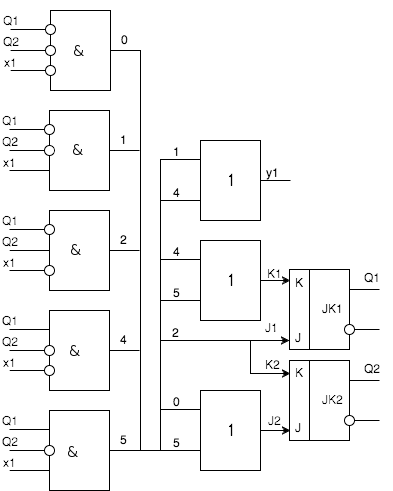
\includegraphics{img/jk.png}

Проверка:
\begin{table}[H]
\tiny
\resizebox{\textwidth}{!}{\begin{tabular}{|c|c|c|c|c|c|c|c|c|}
\hline
\multicolumn{2}{|c|}{Входящий сигнал}        &         & z2 (1)  & z1 (0)  & z1 (0)  & z2 (1)  & z1 (0)  & z1 (0) \\ \hline
\multirow{2}{*}{Состояние}            & Исх. & a1 (00) & a1 (00) & a2 (01) & a3 (10) & a2 (01) & a3 (10) & a1 (00) \\ \cline{2-9}
                                      & Тр.  &         & 00      & 01      & 10      & 01      & 10      & 00 \\ \hline

\multirow{2}{*}{Выходящий сигнал}     & Исх. &         & w1 (1)  & w2 (0)  & w2 (0)  & w2 (0)  & w2 (0)  & w1 (1) \\ \cline{2-9}
                                      & Тр.  &         & 1       & 0       & 0       & 0       & 0       & 0 \\ \hline
\end{tabular}}
\end{table}


\paragraph{T-триггер}\mbox{}\\

По таблице 4, согласно таблицам 1-3 строим таблицу функции
переключения T-триггера:

$T_1T_2 = \mu(Q_1Q_2x_1)$

\begin{table}[!h]
\begin{tabular}{|c|c|c|c|}
\hline
$x_1 \backslash Q_1Q_2$ & $00$ & $01$ & $10$ \\ \hline
$0$          & $01$ & $11$ & $10$ \\ \hline
$1$          & $00$ & $- $ & $11$  \\ \hline
\end{tabular}
\end{table}

ДНФ:

$T_1 = 2 \vee 4 \vee 5$

$T_2 = 0 \vee 2 \vee 5$

В итоге для T-триггера получаем:

$y_1 = 1 \vee 4$

$T_1 = 2 \vee 4 \vee 5$

$T_2 = 0 \vee 2 \vee 5$

Синтезированный структурный автомат в виде комбинационной схемы и памяти:

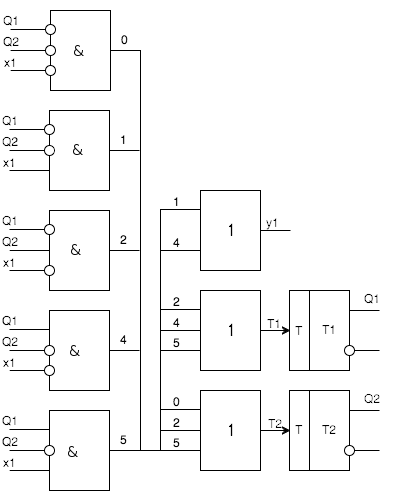
\includegraphics{img/t.png}

Проверка:
\begin{table}[!h]
\tiny
\resizebox{\textwidth}{!}{\begin{tabular}{|c|c|c|c|c|c|c|c|c|}
\hline
\multicolumn{2}{|c|}{Входящий сигнал}        &         & z2 (1)  & z1 (0)  & z1 (0)  & z2 (1)  & z1 (0)  & z1 (0) \\ \hline
\multirow{2}{*}{Состояние}            & Исх. & a1 (00) & a1 (00) & a2 (01) & a3 (10) & a2 (01) & a3 (10) & a1 (00) \\ \cline{2-9}
                                      & Тр.  &         & 00      & 01      & 10      & 01      & 10      & 00 \\ \hline

\multirow{2}{*}{Выходящий сигнал}     & Исх. &         & w1 (1)  & w2 (0)  & w2 (0)  & w2 (0)  & w2 (0)  & w1 (1) \\ \cline{2-9}
                                      & Тр.  &         & 1       & 0       & 0       & 0       & 0       & 0 \\ \hline
\end{tabular}}
\end{table}

\paragraph{D-триггер}\mbox{}\\

По таблице 4, согласно таблицам 1-3 строим таблицу функции переключения
D-триггера:

$D_1D_2 = \mu(Q_1Q_2x_1)$

\begin{table}[H]
\begin{tabular}{|c|c|c|c|}
\hline
$x_1 \backslash Q_1Q_2$ & $00$ & $01$ & $10$ \\ \hline
$0$          & $01$ & $10$ & $00$ \\ \hline
$1$          & $00$ & $- $ & $01$  \\ \hline
\end{tabular}
\end{table}

ДНФ:

$D_1 = 2$

$D_2 = 0 \vee 5$

В итоге для D-триггера получаем:

$y_1 = 1 \vee 4$

$D_1 = 2$

$D_2 = 0 \vee 5$


Синтезированный структурный автомат в виде комбинационной схемы и памяти:

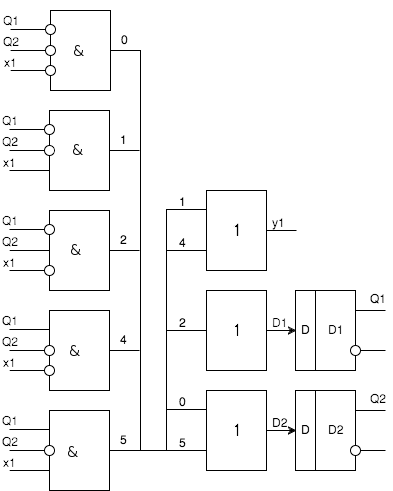
\includegraphics{img/d.png}

Проверка:
\begin{table}[!h]
\tiny
\resizebox{\textwidth}{!}{\begin{tabular}{|c|c|c|c|c|c|c|c|c|}
\hline
\multicolumn{2}{|c|}{Входящий сигнал}        &         & z2 (1)  & z1 (0)  & z1 (0)  & z2 (1)  & z1 (0)  & z1 (0) \\ \hline
\multirow{2}{*}{Состояние}            & Исх. & a1 (00) & a1 (00) & a2 (01) & a3 (10) & a2 (01) & a3 (10) & a1 (00) \\ \cline{2-9}
                                      & Тр.  &         & 00      & 01      & 10      & 01      & 10      & 00 \\ \hline

\multirow{2}{*}{Выходящий сигнал}     & Исх. &         & w1 (1)  & w2 (0)  & w2 (0)  & w2 (0)  & w2 (0)  & w1 (1) \\ \cline{2-9}
                                      & Тр.  &         & 1       & 0       & 0       & 0       & 0       & 0 \\ \hline
\end{tabular}}
\end{table}

\section{Вывод}

В ходе выполнения данной лабораторной работы был изучен метод перехода от
абстрактного автомата к структурному.

\end{document}
